\documentclass[10pt,a4paper]{article}
\usepackage[margin=1in]{geometry}
\usepackage{amsmath,amssymb,booktabs,graphicx}
\usepackage[hidelinks]{hyperref}
\setlength{\emergencystretch}{2em}
\title{Rigid-Block Aggregation for Exact Comparative\\Absolute-Error Optimization on Temporal Networks}
\author{Anonymous technical working draft}
\date{23 November 2026}
\begin{document}
\maketitle
\begin{abstract}
Exact comparative absolute-error optimization over a bounded temporal network
can depend on the smaller group of increasing and decreasing coordinate losses.
That count can be inflated by rigidly related coordinates whose aggregate
slopes cancel. We combine classical rigid-component extraction with complete
aggregate monotonicity classification and conditional extremal extensions.
All nonmonotone blocks and the smaller remaining monotone group are selected,
giving a sufficient parameter that never exceeds the original coordinate count.
Origin-fixed contributions, nonzero flat terms, rational offsets and the
original total-weight normalization are preserved. Equal aggregate endpoint
values are insufficient: a two-coordinate example conceals an interior peak.
With one selected representative, the previous exact original-unary event
sweep remains valid; general fixed dimension retains an XP arrangement bound.
All 380 fixed rational development problems agree with a separate full
original-coordinate oracle and the earlier exact prototype. Sixteen sparse
input-bound checks reach 1024 coordinates, where the parameter falls from
512 to zero or one. Refused and unexecuted baselines are reported separately.
The results concern declared mathematical uncertainty, without a general
complexity classification, solver-superiority claim, physical calibration
or certification of scientific priority.
\end{abstract}
\noindent\textbf{Keywords:} simple temporal networks; rigid components;
absolute-error regret; aggregate monotonicity; exact certificates.
\section{Question and scope}
When baseline and candidate errors are compared at the same uncertain truth,
the worst comparative loss must respect relational constraints between coordinates.
For a closed bounded simple temporal network (STN), a prior exact construction
fixes the smaller orientation group of monotone coordinate losses and fills
the rest by conditional least or greatest feasible extensions. This leaves a
representation issue: many coordinates may be rigidly linked, while their
increasing and decreasing losses cancel after offsets are accounted for.
Treating each coordinate separately can therefore overstate the necessary
search dimension.

We derive a sufficient refined parameter on aggregate block losses, prove
that it cannot exceed the original count, and preserve the original unary
terms in the exact sweep. The refinement does not assume that a block with
different predictions is itself one weighted MAE term. Its classification
requires all feasible kink cells. We then test exactness and audit provenance
on fixed rational cases, with explicit control repairs before the final run.
The scope is a mathematical method extension; it does not estimate unknown
sensor bounds or report a new physical benchmark.
% Body fragment: the including document supplies amsmath and amssymb.
\section{Rigid blocks and comparative absolute error}
\label{sec:rigid-theory}

The rigid-component construction is classical. Theorems~6--7 of
Tsamardinos, Muscettola, and Morris~\cite{tsamardinos1998} directly precede
the SCC characterization and representative/offset substitution below.
Johnson reweighting is likewise classical~\cite{johnson1977}.
We give a self-contained specialization to the declared loss and its
reduction parameter; this attribution is not a novelty certificate.

Let \(I=\{1,\ldots,n\}\), \(I_0=I\cup\{0\}\), and \(t_0=0\).
Assume the finite directed constraints \(t_j-t_i\le b_{ij}\) define a
nonempty bounded set \(S\). All inequalities are non-strict, so \(S\) is
compact. In the arc orientation \(i\to j\), let \(D_{ij}\) be the
shortest-path distance. These distances are finite and satisfy
\[
 D_{ij}=\max_{t\in S}(t_j-t_i),\qquad
 \ell_i=-D_{i0},\quad u_i=D_{0i}.
\]
Indeed every path bounds the difference, while
\(t_j=D_{pj}-D_{p0}\) is an anchored feasible vector attaining each
bound from \(p\). The triangle inequality makes both \(\ell\) and \(u\)
feasible. These are exact marginal endpoints, not independent box
constraints replacing the STN.

For finite fixed \(a_i,c_i\) and \(w_i>0\), put
\[
 f_i(z)=|c_i-z|-|a_i-z|,\quad
 F(t)=\sum_{i\in I}w_i f_i(t_i),\quad
 \Lambda=\sum_{i\in I}w_i,\quad
 W=\max_{t\in S}F(t).
\]
Coordinate 0 has no loss; the comparative MAE is \(W/\Lambda\).
Each unary term is globally monotone. Let \(p_{\rm orig},n_{\rm orig}\)
count its effectively nonconstant increasing and decreasing coordinates,
respectively, and \(r_{\rm orig}=\min(p_{\rm orig},n_{\rm orig})\).
Effective constancy is exactly \(f_i(\ell_i)=f_i(u_i)\).

\subsection{Classical rigid equivalence and offsets}

Choose any feasible potential \(h\), normalized by \(h_0=0\), and form
\(b'_{ij}=b_{ij}+h_i-h_j\ge0\). This arbitrary potential need not be the
forward-0 distance profile. Consider the directed subgraph of exactly
zero reduced-cost arcs.

\noindent\textbf{Lemma 1 (rigid equivalence).}
Its SCCs are precisely the maximal classes for which \(t_j-t_i\) is
constant over \(S\); the constant is \(h_j-h_i\).

\noindent\emph{Proof.}
Zero-cost paths in both directions give the two opposite bounds
forcing equality. Conversely a constant difference has that value
because \(h\in S\). Tightness gives
\(D_{ij}=h_j-h_i\) and \(D_{ji}=h_i-h_j\).
Both reduced shortest-path distances are zero. Nonnegative costs force
zero-length paths to consist entirely of zero-cost arcs.
Thus the vertices lie in one zero-cost SCC. The constant-difference
definition also proves independence from the chosen potential.
\(\square\)

Select a representative \(q_B\) in each block \(B\), with \(q_{B_0}=0\)
for the origin block. Set
\[
 \delta_i=h_i-h_{q_B},\qquad t_i=x_B+\delta_i
 \quad(i\in B).
\]
An arc \(i\in B\to j\in C\) becomes
\[
 x_C-x_B\le b_{ij}+\delta_i-\delta_j.                 \tag{1}
\]
These constraints with \(x_{B_0}=0\) define an exact quotient:
every original truth satisfies them by Lemma~1, and every quotient
truth reconstructs an original truth satisfying every arc by
substitution. Representatives make the correspondence one-to-one.
Internal arcs are automatic; parallel arcs may be replaced by their
minimum bound while retaining original identities.
Consequently
\[
 \begin{aligned}
 D^Q_{BC}&=D_{q_Bq_C},\quad L_B=\ell_{q_B},\quad U_B=u_{q_B},\\
 \ell_i&=L_B+\delta_i,\qquad u_i=U_B+\delta_i .
 \end{aligned}
\]
No argument requires the original truth set to have full dimension.
A single zero-cost arc, or weak connectivity of zero arcs, does not
establish rigid equivalence.

\subsection{Aggregate slopes and the reduction parameter}

For \(B\ne B_0\), define
\[
 A_i=a_i-\delta_i,\quad C_i=c_i-\delta_i,\qquad
 g_B(x)=\sum_{i\in B}w_i\bigl(|C_i-x|-|A_i-x|\bigr).
\]
All members of \(B_0\) are fixed. With
\[
 C_0=\sum_{i\in B_0\cap I}w_i
       \bigl(|c_i-\delta_i|-|a_i-\delta_i|\bigr),
 \qquad F(t)=C_0+\sum_{B\ne B_0}g_B(x_B),             \tag{2}
\]
arbitrary offsets and different unary pairs are preserved exactly.
They need not combine into one weighted absolute-difference term.

On each open segment between shifted kinks, the aggregate slope is
\[
 s_B(x)=\sum_{i\in B}2w_i\operatorname{sign}(a_i-c_i)
  \mathbf{1}_{\{\min(A_i,C_i)<x<\max(A_i,C_i)\}}.     \tag{3}
\]
Inspect all positive-length segments in the exact interval
\([L_B,U_B]\). Let \(\mathcal Z\) contain flat blocks, including
singleton marginals; let \(\mathcal P\) contain nonconstant blocks
whose segment slopes are all nonnegative, and \(\mathcal N\) those
whose slopes are all nonpositive. The remaining blocks
\(\mathcal B\) have slopes of both signs. These cases partition the
nonorigin blocks. Sorting and combining the at most \(2n\) original
events gives the classification in \(O(n\log(n+1))\) arithmetic and
comparison operations.

Endpoint comparison is insufficient: for \(t_1=t_2=x\in[0,2]\),
\(a=(1,1)\), \(c=(0,2)\), and unit weights,
\[
 g(x)=
 \begin{cases}2x,&0\le x\le1,\\4-2x,&1\le x\le2.\end{cases}
\]
Thus \(g(0)=g(2)=0\), whereas \(g(1)=2\).
Flat block values may be nonzero: retain them in (2), or absorb them
into \(C_0\). In either case \(\Lambda\) remains the total original
weight, including all fixed and flat coordinates.

\noindent\textbf{Lemma 2 (parameter domination).}
The aggregate parameter satisfies
\[
 r_\star=|\mathcal B|+\min(|\mathcal P|,|\mathcal N|),
 \qquad r_\star\le r_{\rm orig}.                    \tag{4}
\]

\noindent\emph{Proof.}
Every nonconstant \(\mathcal P\) block contains an effectively
increasing original term, every \(\mathcal N\) block a decreasing
term, and every \(\mathcal B\) block at least one of each.
Otherwise its sum could not have the declared slopes on its exact
marginal. Offsets preserve direction and effective activity.
Blocks are disjoint, so
\[
 |\mathcal B|+|\mathcal P|\le p_{\rm orig},\qquad
 |\mathcal B|+|\mathcal N|\le n_{\rm orig}.
\]
Taking the smaller bound proves (4). \(\square\)

\subsection{Exact conditional representative reduction}

For any selected nonorigin blocks \(K\), define
\[
 Q_K=\{z:L_C\le z_C\le U_C,\
              z_E-z_C\le D^Q_{CE}\ (C,E\in K)\}.
\]
Adjoin \(z_{B_0}=0\), write \(K_0=K\cup\{B_0\}\), and set
\[
 m_B(z)=\max_{C\in K_0}(z_C-D^Q_{BC}),\qquad
 M_B(z)=\min_{C\in K_0}(z_C+D^Q_{CB}).               \tag{5}
\]
For empty \(K\) these are \(L\) and \(U\).

\noindent\textbf{Lemma 3 (conditional extrema).}
\(Q_K\) is the exact projection of the quotient STN.
For every \(z\in Q_K\), both extensions in (5) are feasible, agree
with \(z\) on \(K\), and bound every matching feasible \(x\) as
\(m(z)\le x\le M(z)\).

\noindent\emph{Proof.}
Projected inequalities bound all branches at a selected block, and
its own branch gives equality. The triangle inequality yields
\[
 z_C-D^Q_{EC}\le z_C-D^Q_{BC}+D^Q_{BE}
                   \le m_B+D^Q_{BE};
\]
taking the maximum proves feasibility of \(m\).
If \(C\) attains \(M_B\), then
\(M_E\le z_C+D^Q_{CE}\le M_B+D^Q_{BE}\), proving the other case.
Any matching feasible \(x\) lies above each lower branch and below
each upper branch. Necessity of \(Q_K\) is immediate; the extensions
prove sufficiency. This also handles lower-dimensional domains.
\(\square\)

\noindent\textbf{Theorem 1 (block-minority reduction).}
If \(|\mathcal P|\le|\mathcal N|\), choose
\(K=\mathcal B\cup\mathcal P\). Then
\[
 W=\max_{z\in Q_K}\left[C_0+
                  \sum_{B\ne B_0}g_B(m_B(z))\right].              \tag{6}
\]
For \(|\mathcal N|\le|\mathcal P|\), choose
\(K=\mathcal B\cup\mathcal N\) and use \(M\).

\noindent\emph{Proof.}
In the first case, all nonmonotone and increasing block losses are
fixed on a fibre. Remaining nonconstant losses are nonincreasing,
so the least extension maximizes their sum on that fibre.
It is feasible, and the projection is exact; maximizing proves
(6). The greatest-extension case is symmetric. Compactness gives
attainment, and offsets reconstruct an original worst truth.
\(\square\)

For \(r_\star=0\) the appropriate endpoint extension suffices,
even when original individual directions are mixed.
This parameter is a sufficient reduction size, not a claim of
minimal possible dimension.

\subsection{One representative and strict separation families}

For \(r_\star=1\), let \(p\) be the selected representative.
Using original distances and original unary terms, the path is
\[
 t_i(z)=\max(\ell_i,z-D_{ip})
 \quad\hbox{or}\quad
 t_i(z)=\min(u_i,z+D_{pi}),\qquad z\in[\ell_p,u_p].   \tag{7}
\]
These formulas enforce all offsets automatically. They remain
valid when the selected block loss is nonmonotone.
Put \(l_i=\min(a_i,c_i)\), \(v_i=\max(a_i,c_i)\).
On the least path, a nonconstant term has slope
\(s_i=2w_i\operatorname{sign}(a_i-c_i)\) between
\[
 \max(\ell_i,l_i)+D_{ip}\quad\hbox{and}\quad v_i+D_{ip};
\]
skip \(a_i=c_i\) or \(\ell_i\ge v_i\).
On the greatest path the event interval is
\[
 \bigl(l_i-D_{pi},\,\min(u_i,v_i)-D_{pi}\bigr);
\]
skip \(a_i=c_i\) or \(u_i\le l_i\).
Each original term has at most two events. Between consecutive
events the objective is affine, so an endpoint or event attains
the maximum: at most \(2n+2\) candidates before deduplication.
Initialize the right slope at the left domain endpoint, combine
simultaneous events, and evaluate each event before updating its
slope. No grid is required. Given the required profiles, the
mathematical sweep takes \(O(n\log(n+1))\) operations and \(O(n)\)
extra storage. Checking its witness against all \(M\) original arcs
gives \(O(M+n\log(n+1))\) postprocessing, excluding preprocessing.

Two analytical families give strict separation from the original
coordinate parameter. Let \(n=2m\), all truths equal
\(x\in[0,2]\), and all weights be one.
Repeating \(m\) pairs \(a=(1,0)\), \(c=(0,1)\) cancels identically:
\[
 r_{\rm orig}=m,\qquad r_\star=0,\qquad W=W/\Lambda=0.
\]
Repeating \(m\) pairs \(a=(1,1)\), \(c=(0,2)\) gives the peak above:
\[
 r_{\rm orig}=m,\quad r_\star=1,\quad
 W=2m\ \hbox{at }x=1,\quad \Lambda=2m,\quad W/\Lambda=1.
\]
Arbitrary rigid offsets preserve these identities when the same
offset is added to each truth, baseline, and candidate entry.
The displayed values assume unit weights; arbitrary positive
weights are permitted by the theorem but need not preserve
cancellation. This compares with the unreduced coordinate
parameter, not every classical presolver, and reports no experiment.

Interior alternatives use pairs \(a=(3/2,1/2)\), \(c=(1/2,3/2)\)
for cancellation, or \(a=(1,1)\), \(c=(1/2,3/2)\) for the peak.
The latter pair is zero outside \([1/2,3/2]\), rises with slope 2
to height 1 at \(x=1\), then falls with slope \(-2\).
Thus the respective \(r_\star\) values remain 0 and 1; the peak
family has \(W=m\) and \(W/\Lambda=1/2\).
Both alternatives have \(k=\#\{i:\ell_i<c_i<u_i\}=n\).
This separates the parameters, not LP running times or lower bounds:
common-truth families have few distinct levels and feasible sign patterns.

\subsection{General dimension, implementation scope, and checking}

For \(r=r_\star\ge1\), partition \(Q_K\) by equalities between
conditional affine branches, their crossings of every shifted
original unary kink, and projected-domain boundaries.
Discard constant equalities and combine duplicate hyperplanes.
With \(b\) blocks, there are
\(H=O(br^2+nr+r^2)=O(nr^2)\) hyperplanes.
The objective is affine on each cell closure, so some optimum is a
cell vertex. Enumerating \(r\) independent active hyperplanes,
checking the projection, and evaluating the extension gives
\[
 O\!\left(H^r(r^3+r^2+nr)\right)
\]
arithmetic complexity. Domain equalities supply missing normals
in lower-dimensional cases. This is XP for fixed \(r\), not FPT
or general polynomial time. Incomplete enumeration does not certify
an optimum.

Distance profiles in the intended implementation remain on the
\emph{original graph}. The quotient supports classification,
representative selection, and the equivalence proof; no fully
contracted shortest-path solver is presumed. Classical feasible
potentials and forward/reverse Dijkstra require \(2r+2\) profiles.
Reverse the already reweighted graph, and retain original identities
when coalescing parallel arcs. With \(M\) original input arcs, a
safe preprocessing and classification bound is
\[
 O\!\left(nM+(r+1)(M+n)\log(n+1)+n\log(n+1)\right),
\]
with \(O(M+(r+1)n)\) storage. The Bellman--Ford term remains.

Independent checking is a separate obligation: validate input
binding, potential, SCCs, offsets, every aggregate slope segment
and constant, selected representatives, required distance profiles,
complete sweep or arrangement coverage, original feasibility,
objective, and original normalization. A feasible witness alone
gives only a lower bound on \(W\). No checker execution or pass is
asserted here. Exact arithmetic bounds do not remove rational bit
costs; real inputs require an exact-real interpretation.
Floating-point zero tests do not certify rigid contraction.
The result establishes no new shortest-path method, general
polynomial or FPT algorithm, physical accuracy, or publication-level
novelty.


\section{Recorded exact checks}
\label{sec:checks}
The development protocol freezes all source, rational inputs and theoretical
source fragments before the actual run. The 380 inputs comprise 224 unchanged
parent regression problems with prefixed identifiers, 144 new problems
(48 graph/offset configurations with three policies each), and 12 named guards.
New random configurations use two to four original coordinates, origin-fixed
members, nonzero rational offsets, directed rigid cycles, unequal weights,
parallel arcs and one-way tight edges. Named guards cover aggregate cancellation,
nonzero flat values, a hidden interior peak, fixed-origin constants and two
nonmonotone blocks. These are designed development cases, not independent
physical samples or a preregistered evaluation.

A separate verifier imports no producer numerical code. It uses mutual
reachability rather than the producer SCC routine, and evaluates original
unary functions at every block kink to compute secant slopes rather than
reusing slope-event accumulation. Source-zero distance inequalities and rooted
tight trees with original arc identities certify every required profile.
It reconstructs the selected block representatives, offsets, quotient arcs,
constant contribution, original normalization and returned conditional truth.
For one representative it independently evaluates a complete original-unary
critical-point superset and checks all reported sweep segments and bends.

For every development input, an additional oracle enumerates full-rank
original-coordinate intersections of original constraint boundaries and unary
kinks, using exact spanning-tree potentials. It filters by all original
constraints and evaluates the actual weighted loss. Compactness and the affine
cell argument ensure an original-coordinate optimum is included. This oracle
uses neither the producer reduction nor its SCC, sparse shortest-path or sweep
implementation. All 380 optimum values and returned truths passed. The original
coordinate prototype also returned the same exact values on all 380 cases.
This is separate implementation evidence for a shared mathematical definition,
not an independently measured physical truth.

The structural modes were endpoint 233, sweep 140
and reduced arrangement 7.
The parameter decreased strictly on 52 cases,
was unchanged on 328 and never increased.

For dimensions above one, the original-coordinate oracle checks the optimum
and witness; it does not certify the compressed plane/basis inventory as a
standalone complete proof. Offline replay reproduced all deterministic results
and repeated the same original-coordinate oracle. Repeated inputs are not
counted as new independent samples.

\paragraph{Controls and repairs before the freeze.}
The first root control attempt supplied Fraction objects where canonical
rational strings were required; parsing rejected it before optimization.
After correcting this driver fixture, all 12 named controls and eight analytical
value checks passed. Earlier source bytes and the failure receipt were preserved.
The independent checker rejected 26 actual mutations. Separate inventory guards
rejected duplicated, missing and reordered cases. A conflicting earlier hash
was also rejected rather than overwritten by a current hash for the same path.
Native criticism found the latter two provenance gaps before the actual run:
the verifier originally checked row count without frozen input identities,
and a last-wins binding merge could discard the frozen expected hash.
Both were repaired before execution. Exact input identities, order, uniqueness,
cardinality and all original frozen bindings are now checked explicitly.
All recorded control revisions include source snapshots. Native AI criticism
is bounded review evidence, not human peer review.

\section{Sparse parameter study}
\label{sec:benchmark}
We instantiate interior variants of the two families in Section~\ref{sec:rigid-theory}
at $n=4,16,128,1024$, with signed rational offsets and sparse directed rigid
cycles. Cancellation uses pairs $a=(3/2,1/2)$, $c=(1/2,3/2)$; the peak uses $a=(1,1)$, $c=(1/2,3/2)$. Each is evaluated at scales 1 and $10^6$, giving 16 configurations
from eight structures. Every candidate kink lies strictly inside its original
marginal, so the candidate-sign count is $k=n$; nevertheless the actual feasible
sign patterns in this common-truth family are few. This is a separation of
declared parameters, not an exponential lower bound or evidence against a
presolved LP formulation.

Each generated input is saved and hashed before analysis. Original-graph
analysis includes feasible-potential preparation, origin profiles, iterative
zero-edge SCCs, aggregate classification, quotient evidence and the selected
profiles. Optimization uses the previous exact original-unary sweep or
arrangement code after this new selection, including certificate construction
and an original-arc feasibility check. We record analysis once and the median
of three post-warmup optimization observations. Timings are dependent observations
on one concurrently used Windows machine running Python 3.11.0rc2; no confidence
interval or fitted complexity exponent is claimed.

\begin{table}[ht]
\centering\small
\caption{Recorded scale-1 phase times in milliseconds. Refusals and unexecuted
baselines are categorical outcomes, not comparative solution times. All16
scale-1 and scale-$10^6$ records are preserved in the package.}
\begin{tabular}{rlrrrrl}
\toprule
$n$ & Family & $r_{\rm orig}$ & $r_\star$ & Analysis & Optimize & Original prototype\\
\midrule
4 & cancellation & 2 & 0 & 1.121 & 0.077 & exact \\
4 & peak & 2 & 1 & 0.895 & 0.236 & exact \\
16 & cancellation & 8 & 0 & 3.219 & 0.285 & budget refusal \\
16 & peak & 8 & 1 & 2.426 & 0.554 & budget refusal \\
128 & cancellation & 64 & 0 & 15.609 & 2.145 & not run \\
128 & peak & 64 & 1 & 20.580 & 5.691 & not run \\
1024 & cancellation & 512 & 0 & 130.844 & 17.829 & not run \\
1024 & peak & 512 & 1 & 267.992 & 63.090 & not run \\
\bottomrule
\end{tabular}
\end{table}

The original prototype was actually run only at $n\le16$, with its complete
arrangement preflight budget of 1000 bases. Four configurations completed
exactly and four refused before enumeration. The eight configurations with
$n>16$ were not executed under that size policy. The displayed lower bound
$\binom{2r_{\rm orig}}{r_{\rm orig}}$ follows from distinct lower/upper domain
planes; it is theoretical and is not a measured refusal. No value is reported
from an incomplete search. No optimized published solver or candidate-sign
LP family was timed, and there is no solver-superiority claim.

All16 structural results passed a separate original-input-bound checker.
This combines independently reconstructed maximal rigid classes and aggregate
secants with profile trees and original-unary endpoint/event optimality checks;
it does not enumerate a 1024-dimensional truth arrangement. The independent
checker uses $O(n(n+M))$ arithmetic/comparison operations and $O(n^2+M)$ storage
for mutual reachability and direct cell checks. Those costs are distinct from
producer preprocessing and sweep costs. All eight scale pairs preserved the
block partition and scaled the optimum exactly. This is not timing invariance.
The $n=1024$ cases have $r_{\rm orig}=512$ but $r_\star=0$ or 1, and use two
or four actual profiles instead of the original prototype's theoretical 1026.

\begin{figure}[ht]
\centering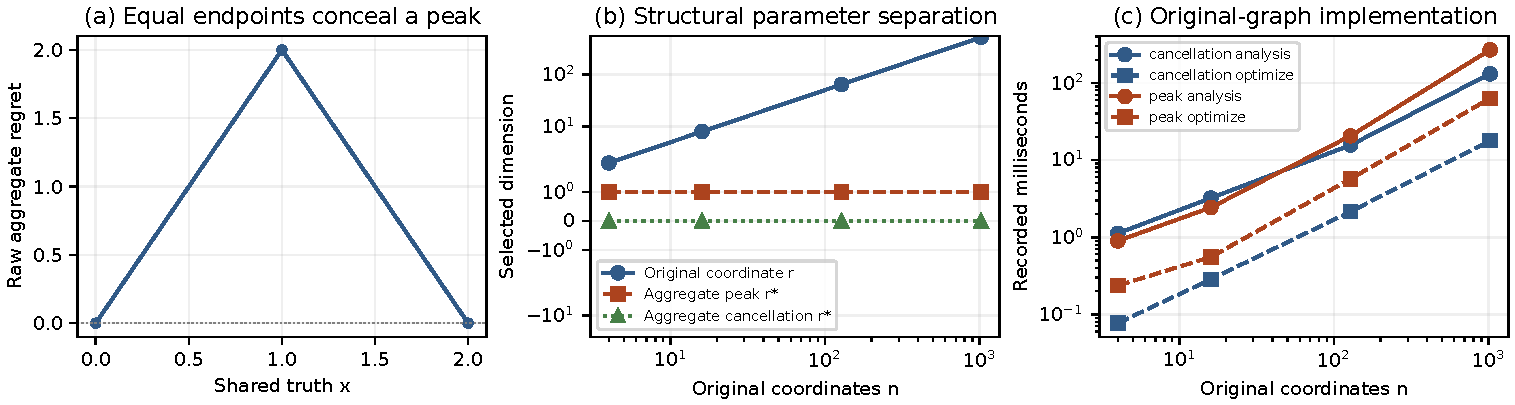
\includegraphics[width=\linewidth]{figure1.pdf}
\caption{The endpoint-equality guard, parameter separation, and recorded
scale-1 timings. The peak in (a) is a named development guard; the interior
benchmark pair has height one. In (c), lines guide the eye without fitting
a complexity law.}
\end{figure}

\section{Interpretation, reproducibility and submission status}
The concrete refinement is complete aggregate monotonicity after classical
rigid contraction, with mandatory selection of all nonmonotone blocks.
It removes arbitrary inflation of the original direction count on the displayed
offset/cancellation families. A representative is a coordinate parameter,
not a new independent observation. Rigid SCC extraction and offset substitution
are direct classical antecedents \cite{tsamardinos1998}; earliest/latest and
partial-assignment temporal bounds are also established \cite{dechter1991}.
The bounded prior review does not certify priority of this specialization.

General piecewise-linear temporal preferences have substantial precedent
\cite{kumar2007,kumar2018}. Concave utility results and historical conjectures
must not be turned into a general polynomiality or hardness claim for the
present objective. The bound is still XP in $r_\star$, and this parameter need
not be the smallest possible reduction dimension. Rational bit costs and
floating-point zero robustness remain separate from exact operation counts.

The source/result package contains every actual input, result and oracle row,
pre-analysis large input hashes, all control source snapshots, fixed bindings,
literature acquisition limits and an offline replay entry point. A SHA-256
index checks every archive member byte; no archived code is executed when
building or verifying that archive. Recorded replay instead uses reviewed
local sources, without historical Orca state, parent result files, network
or model calls. Preserving the documented outputs/study directory layout is
required for its relative source bindings. Primary paper bytes were not
collected by this review; note hashes authenticate notes, not original PDFs.
Johnson's full original article remains uninspected.

The guarantee is conditional on the supplied nonempty bounded closed STN.
No new sensor/reference/alignment calibration or external holdout was obtained,
and the previous empirical failure is not repaired or reclassified by these
mathematical results. Human proof review, publishable-contribution and priority
judgment remain outstanding. Existing manuscripts are preserved separately.

\paragraph{Author and submission facts.}
AI assistance was substantial in derivation, coding, checking and writing.
Exact service/model revision, responsible human authors and order,
affiliations, correspondence, funding, interests, public data/code destination,
originality declarations and final human approval remain unconfirmed.
No values are invented for these fields. This is an anonymous technical
extension, not a submitted or submission-ready manuscript.

\section*{Acknowledgements}
This work was created as part of the No-More-Slops group activities at Pseudo Lab.

\begin{thebibliography}{9}
\bibitem{tsamardinos1998} I.~Tsamardinos, N.~Muscettola and P.~Morris.
Fast transformation of temporal plans for efficient execution. \emph{AAAI} (1998).
\bibitem{dechter1991} R.~Dechter, I.~Meiri and J.~Pearl.
Temporal constraint networks. \emph{Artificial Intelligence} 49 (1991), 61--95.
\bibitem{johnson1977} D.~B.~Johnson. Efficient algorithms for shortest paths
in sparse networks. \emph{Journal of the ACM} 24(1) (1977), 1--13.
\bibitem{kumar2007} T.~K.~S.~Kumar. Fast (incremental) algorithms for useful
classes of simple temporal problems with preferences. \emph{IJCAI} (2007).
\bibitem{kumar2018} T.~K.~S.~Kumar, Z.~Wang, A.~Kumar, C.~M.~Rogers and C.~A.~Knoblock.
Load scheduling of simple temporal networks under dynamic resource pricing.
\emph{AAAI} (2018).
\end{thebibliography}
\end{document}
